\setlength{\fboxsep}{0pt}
\setlength{\fboxrule}{1pt}
\begin{figure}[H]
	\centering
	\begin{subfigure}[t]{0.48\linewidth}
		\centering
		\fbox{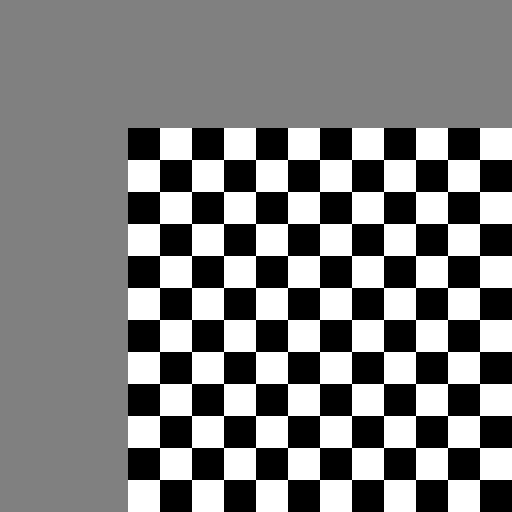
\includegraphics[width=0.48\textwidth]{Figures/Example/exampleV.png}}
		\caption{Noise-free image $V$.}
		\label{fig: exampleV}
	\end{subfigure}
	\hfill
	\begin{subfigure}[t]{0.48\linewidth}
		\centering
		\fbox{
\includegraphics[width=0.48\textwidth]{Figures/Example/exampleF.png}}
		\caption{Noisy data $F$ with underlying ground truth $V$ and standard deviation $\sigma = 55$.}
		\label{fig: exampleF}
	\end{subfigure}
	\vfill
	\begin{subfigure}[t]{0.48\linewidth}
		\centering
		\fbox{
\includegraphics[width=0.48\textwidth]{Figures/Example/exampleI.png}}
		\caption{Image after binarization through the statistical test.}
		\label{fig: exampleI}
	\end{subfigure}
	\hfill
	\begin{subfigure}[t]{0.48\linewidth}
		\centering
		\fbox{
\includegraphics[width=0.48\textwidth]{Figures/Example/exampleI_o.png}}
		\caption{Image after binarization and morphological opening.}
		\label{fig: exampleI_o}
	\end{subfigure}
	\vfill
	\begin{subfigure}[t]{0.48\linewidth}
		\centering
		\fbox{
\includegraphics[width=0.48\textwidth]{Figures/Example/exampleI_oc.png}}
		\caption{Image after binarization, morphological opening and closing.}
		\label{fig: exampleI_oc}
	\end{subfigure}
	\caption{Example of an image and the extraction of the ROI through the statistical test and morphological operations. Images are $16 \times 16$ pixels ($\alpha = 0.05, \varphi = 5$).}
	\label{fig: example}
\end{figure}